\subsection{Appendicitis Patient Length of Stay}
This section and demonstrates the potential of pathway performance analysis based on the identified pathway variants. Patient length of stay at each stage of the appendicitis pathway measured from admission for all patient traces that follow the first pathway variant (index 0) and the third pathway variant (index 2) are shown in Fig.~\ref{fig:appendicitis length of stay variant 0} and Fig.~\ref{fig:appendicitis length of stay variant 2} respectively. These plots could be useful for identifying potential rate-determining steps in a healthcare pathway. One patient trace from Fig.~\ref{fig:appendicitis length of stay variant 0} and six patient traces from Fig.~\ref{fig:appendicitis length of stay variant 0} have unusually long surgery waiting times. The number of patient traces that follow each pathway variant is limited for this study, and more samples are required to confirm causes of delay along the appendicitis pathway. 

\begin{figure}[t]
    \centering
    \begin{minipage}{0.48\textwidth}
        \centering
        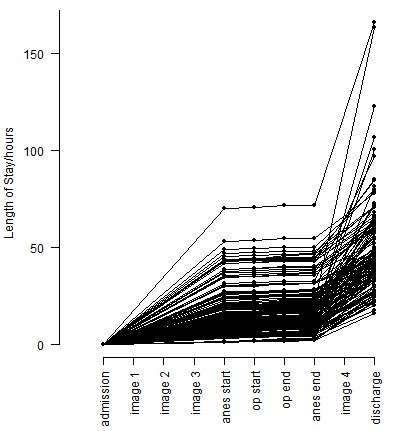
\includegraphics[width=\textwidth]{images/appendicitis_variant_length_of_stay_0_journal.jpg}
        \caption{Hospital length of stay of appendicitis patient traces following pathway variant 0. There is one potential outlier for surgery waiting time.}
        \label{fig:appendicitis length of stay variant 0}
    \end{minipage}\hfill
    \begin{minipage}{0.48\textwidth}
        \centering
        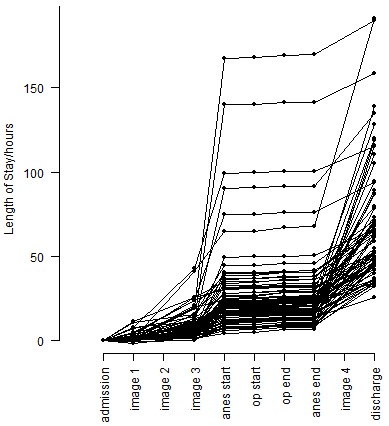
\includegraphics[width=\textwidth]{images/appendicitis_variant_length_of_stay_2_journal.jpg}
        \caption{Hospital length of stay of appendicitis patient traces following pathway variant 2. There are six potential outliers for surgery waiting time.}
        \label{fig:appendicitis length of stay variant 2}
    \end{minipage}
\end{figure}